%% chapter of SNO+ detector

%%\epigraph{There is an art in the contemplation of water. It is necessary to look at it as foaming in waves.}{--- \textup{Mencius}, \textit{\\translated by James Legge}}


\section{A Description of SNO+ Detector}

\subsection{Overview}
The SNO+ experiment is located at SNOLAB in Vale's Creighton mine in Sudbury, Ontario, Canada. The deep underground facility of the SNOLAB provides a $2092\pm6$ m flat overburden of rock, which is $5890\pm94$ water equivalent meter (w.e.m). This rock overburden ensures an extremely low rate of cosmic muons passing through the detector. The rate is $0.27~\mu/m^2/day$, compared to an average flux of about $1.44\times 10^6~\mu/m^2/day$ at sea level\cite{muonflux}.

The detector has been running since December 2016\cite{ndpaper},


The SNO+ detector is the successor of the SNO experiment, which makes use of the SNO detector structure. 


detector consists of an acrylic vessel (AV) sphere of 12 m in diameter and

5.5 cm in thickness. The AV sphere is concentric within a stainless steel photomultiplier(PMT) support structure (PSUP), with an average radius of 8.4 m. The Hamamatsu 8-inch R1408 PMTs are mounted on the PSUP. 9394 PMTs are looking inward to the AV, giving a 50\% effective coverage, while 90 PMTs are looking outward, serving as muon vetos. These two structures are housed in a rock cavity filled with 7000 tonnes of ultrapure water (UPW) to provide both buoyancy for the vessel and radiation shielding.


main upgrades from SNO to SNO+
BiPo tagging on partial fill data

\subsection{SNO+ Physics Phases}
The SNO+ detector is designed for multi-purpose measurements of neutrino physics.
The experiment will go through three phases\cite{whitepaper}: 

1. Water phase 

The AV was filled with about 905 tonnes of ultra pure water (UPW). The detector has been collecting physics data since May 2017.

The main physics goal in this phase is to search for the invisible nucleon decay, which violates baryon number and is a prediction of Grand Unified Theory (GUT). In this decay mode, $^{16}$O decays into $^{15}$O$^*$ or $ ^{15}$O$^*$, which de-excites and produces a $\gamma$ ray of about 6 MeV.

During the water phase, different types of calibration runs have been taken. The detector responses, systematics and backgrounds are studied. Multiple physics analyses of solar neutrinos, reactor antineutrinos and nucleon decay are going on. The external backgrounds are also measured, which will be the same as the following two phases. 

2. Scintillator phase

The AV will be filled with 780 tonnes of liquid scintillator, which is a mixture of linear alkylbenzene (LAB) as a solvent and 2 g/L of 2,5-diphenyloxazole (PPO) as a fluor.

In this phase, the main physics goal is to measure low energy solar neutrinos: the CNO, pep and low energy $^8$B neutrinos. The pep neutrinos are mono-energetic, with $E_\nu$=1.442 MeV and their flux is well predicted by the Standard Solar Model. A measurement of the pep neutrinos will give more information of the matter effects in neutrino oscillations\cite{borexino}. 

The solar metallicity is the abundance of elements heavier than $^4$He (called ``metal'' elements in the context of astronomy). It is poorly constrained and the predictions from different solar models disagree with each other. A measurement of the CNO neutrinos can give the abundance of $^{12}$C, $^{13}$N and $^{15}$O and can thus resolve the metallicity problem\cite{cno}.

Geoneutrino, reactor antineutrino and supernova neutrino detections are additional goals.

A six-month period of scintillator filling and six to twelve months of data-taking are expected for this phase. During the filling, it is planned to operate the partially filled detector at a water level about 4.4 m for about two weeks. This partial filled transition phase is mainly aimed to understand the in-situ backgrounds of scintillator. 

3. Tellurium loading phase

In this final phase, 0.5\% natural Tellurium by mass will be loaded into the scintillator.
Higher loading concentrations would be possible for a further loading plan\cite{Paton:2019kgy}.
 The $^{130}$Te is a double beta decay isotope. The main purpose in this phase is searching for $0\nu\beta\beta$ in $^{130}$Te.


\subsection{Detection Principle}

\subsubsection{Optical Cherenkov Radiation Detection}
In the SNO+ water phase, the relay on the .

For any charged particle travelling in a transparent medium at an ultrarelativistic speed (a speed greater than the local phase speed of light in the medium), there is an electromagnetic radiation emitted from the medium under the action of the field of the moving particle\cite{landau2013electrodynamics}.


\[v>v_p=c/n(\omega)\]   $\cos\theta_c = (1/n\beta)$


where c is the speed of light in vacuum, n is the refraction index of the medium and $v=\beta c$ is the speed of the particle in the medium.


Frank-Tamm formula

For a particle with a charge of $ze$, the number of photons produced by Cherenkov radiation per unit path lenght and per unit energy interval of the photons is described by :
 
\[
\frac{d^2N_r}{dEdx}=\frac{\alpha^2 Z^2}{\hbar c}\mu(E)(1-\frac{1}{\beta^2 n(E)^2})
\]

where $\alpha$ is the fine structure constant



For the case of $e^-$ travelling in the water, we can find that 0.262 MeV is the lowest kinetic energy to create Cherenkov radiation, which is called the Cherenkov threshold.

\subsubsection{Scintillation Detection}

prompt emission of scintillation light, which is called fluorescence
delayed emission of scintillation light, which is called delayed fluorescence or phosphorescence.

\subsection{Electronics}

The SNO+ electronics system includes trigger and readout systems, which record the time and charge information of PMT signals. The system can measure signals with a nanosecond-level timing resolution and single-photon level charge resolution and handle a rate of several kHz for normal operations.

burst 
from supernova









PMTs are Hamamatsu model R1408.


a single RG59/U type 75 $\Omega$ coaxial cable

19 crates$\times$16 cards$\times$32 channels = 9728 electronics channels.

Each crate processes 16$\times$32 = 512 PMTs.
9605 channels are actually used and among them, 32 channels are reserved for calibration devices and labelled as FEC Diagnose (FECD) channels


During the experiment running, the maintenance of the electronics is always ongoing.

crate controller card (XL3)


analog master trigger system (MTC/A+) 
("+" means an upgrade to SNO MTC/A)


digital master trigger system (MTC/D)

the analog waveforms are summed on the MTC/A+ card, then they are digitized 

CAEN v1720 digitizer 

TUBii trigger utility board 
pulsers and delays

DAQ 


nearline provides a real-time analysis of the data quality, 

trigger system
PMT Interface Card (PMTIC)
Front End Card (FEC)

NHit20 (N20), NHit100 (N100) trigger pulses.

MTC/A has 3 discriminators: LOW, MED and HI.

Global Trigger (GT)
the timing and charge from the fired PMT is digitized and stored.




Nhit means the number of live hit PMTs in the detector for a given event.


dark noise rate is estimated to be 1 kHz.



\subsection{Optics}

Optical parameters

Winston cone



timing


attenuation

scattering


laser pulse diffuser, it can run with different wavelengths: 337, 365, 385, 420, 450 and 500 nm.
The laserball 

The acrylic of the AV is UV-transparent



\subsection{Liquid scintillator}


Linear Alkyl Benzene (LAB)

is provided by CEPSA Qu\'{i}mica B\'ecancour Inc.
Organic liquid scintillators 
The advantages of LAB are:

\begin{itemize}
	\item[$\bullet$] It has very low levels of natural radioactive contaminants such as U, Th and K.
	\item[$\bullet$] High light yield and attenuation length.
	\item[$\bullet$] It has fast timing response 
	different timing spectrum for $\alpha$ and $\beta$ events, which enables an $\alpha-\beta$ discrimination. 
	\item[$\bullet$] High flash point and low toxicity for lab safety.
	\item[$\bullet$] appropriate density for mechanical stability
	\item[$\bullet$] Good stability and chemically compatible with detector materials, mainly the AV.
	\item[$\bullet$] Low cost.
\end{itemize}


Te-loaded liquid scintillator (TeLS)

To load the tellurium into the liquid scintillator, a compound is made by 
condensation reactions between telluric acid (TeA) and 1,2-butanediol (BD), with N,N-dimethyldodecylamine (DDA) being used as a stabilization agent.


2 g/L PPO gives an absolute light yield of 11900 photons/MeV.


for the partial-fill phase, 0.5 g/L PPO gives Measurements in 0.5 g/L showed a light yield of 52\% of 2 g/L,  
6190 photons/MeV\cite{joshW1,tanner0p5}.

	
\begin{figure}[!htb]
	\centering
	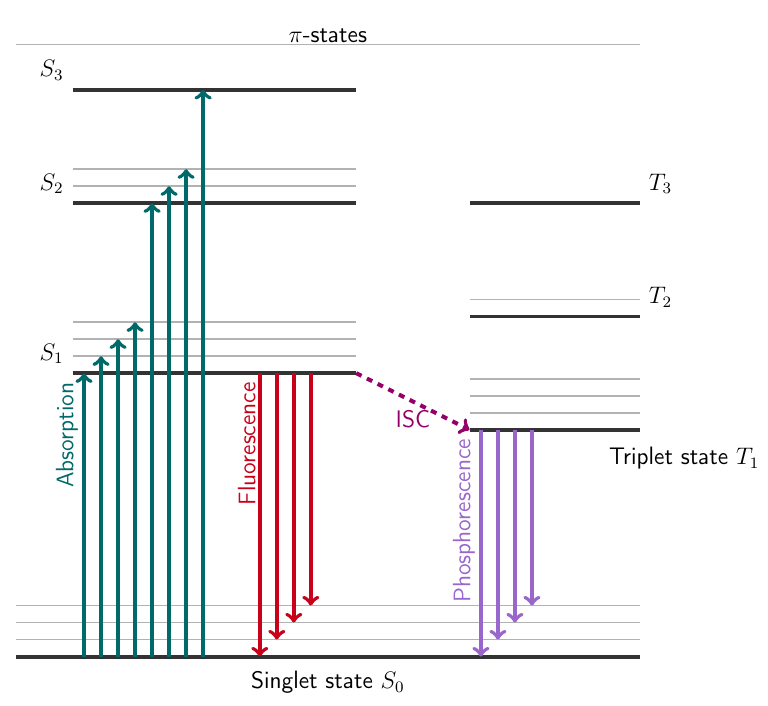
\includegraphics[width=10cm]{jablonski.png}
	\caption{A Jablonski diagram for the liquid scintillator, modified from \cite{knoll2010radiation,birks1965theory}.}
	\label{jablonski}
\end{figure}




Tellurium-loaded 65\% of the pure, unloaded scintillator



water-based wavelength shifter


timing profile, the intensity of scintillation light as a function of time

the prompt fluorescence intensity at a time $t$ excitation be $I=I_0e^{-\frac{t}{\tau}}$



singlet and triplet states 
ionization density 
depend
$\alpha$-particle
high ionization density 
quenching, 


\subsection{Calibration}


Two kinds of calibration sources are used by SNO+: optical sources and radioactive sources. 
The optical sources are used to calibrate the PMT response and to measure the optical properties of the 


The radioactive sources are used to calibrate the energy 

reconstruction performances and uncertainties.
particle identifications







Calibration sources with known physics parameters: help to
understand the detector response to the events and to make
accurate measurements
Two types of SNO+ calibration sources: optical sources and
radioactive sources
Optical sources: phototube response, optical properties of the
detector media
Radioactive source: energy scale, resolution, systematic
uncertainties
16N calibration source is one of the radioactive sources







Optical calibration  {\emph {in-situ}} 
\begin{itemize}  
	\item[$\bullet$] Timing module for the Embedded LED Light Injection Entity (TELLIE)
	
	light-emitting diode (LED)
	
	
	time calibration, time response 
	
	a precision of $\mathcal{O} (1~ns)$
	
	Blinky fibre optics nailed to the PSUP to calibrate stuff.
	
	
	
	\item[$\bullet$]  
	
	
	\item[$\bullet$] 
\end{itemize}





Calibration source

The $^{16}$N source
$^{3}$H$(p,\gamma)^{4}$He reaction.

the SNO+ Source Manipulator System (SMS)
is inherited from the SNO.



A Umbilical Retrieval Mechanism (URM) is used to send the source down to the inner vessel.



The sources are connected to the umbilical.


An umbilical encloses electrical cables, optical fibres and gas lines connected to the source.

A Universal Interface (UI) connecting the URM and the detector, 
Therefore, sealed environment, which 
ensures radon gas not leaking into the detector when deploying the source.

-






